\section{Introduction}
\PARstart{V}{ision} depends on an uninterrupted chain of structures: the retina, the optic nerve, the optic chiasm, the lateral geniculate nucleus, the optic radiations and the visual cortex. A lesion anywhere along the chain can degrade sight, and the clinical picture depends on where the damage lies and on whether it disturbs the anatomy, the conduction of the electrical signal, or both. Glaucoma, a progressive optic neuropathy, had an estimated global prevalence of 3.54\% among people aged 40 to 80 years, or about 64.3 million people in 2013 \cite{tham2014}, and its degeneration extends to the intracranial optic nerve, the lateral geniculate nucleus and the visual cortex \cite{gupta2006}. Optic neuritis is characterised electrophysiologically by a delayed P100 peak of the visual evoked potential (VEP) \cite{halliday1972}, and cortical visual impairment (CVI) arises from damage to the brain's visual pathways \cite{sakki2018}.

Two investigations are routinely used to examine this pathway, and they answer different questions. Structural MRI gives a three-dimensional picture of anatomy, so that atrophy and focal lesions can be localised, but it carries no timing information. The VEP is a one-dimensional recording whose latency and amplitude, in particular those of the P100 component, reflect conduction in the pathway \cite{odom2016}, but it carries no spatial localisation. Combining complementary modalities has long been proposed as a way to reveal relationships that no single modality shows \cite{calhoun2016}.

Learning such a combination faces four obstacles. Most pipelines analyse only one modality (\emph{unimodal isolation}). A volume and a waveform differ in dimensionality, sampling and noise, and simple fusion by concatenation gives every feature the same standing (\emph{cross-modal heterogeneity}). A black-box classifier is difficult to trust clinically (\emph{limited interpretability}). Finally, no public dataset offers paired MRI, VEP and diagnosis labels (\emph{the labelling gap}). Published multimodal fusion studies with cross-attention \cite{zhou2024camf,dhar2025drifa} also tend to report a single headline number, which makes it hard to tell \emph{when} fusion is responsible for a gain.

This paper presents the Cross-Attention Fusion Network (CAFN) and, more importantly, an evaluation designed to answer that question honestly in a setting where real paired data are scarce. The contributions are:
\begin{enumerate}
\item \textbf{Architecture.} CAFN couples a squeeze-and-excitation 3D residual encoder and a multi-scale 1D encoder through \emph{gated bidirectional} cross-attention (each stream queries the other), with learned attention pooling, positional embeddings and two auxiliary unimodal heads. All pooling is implemented with deterministic matrix products, so GPU training is reproducible.
\item \textbf{A controlled benchmark of when fusion helps.} A synthetic generator with independent knobs for the class information carried by each modality allows a like-for-like comparison of cross-attention against concatenation, element-wise sum and unimodal models, a component ablation of seven design choices, and a sweep over modality informativeness, all with multiple seeds and a held-out test set.
\item \textbf{A reproducible real-data protocol.} A one-command pipeline downloads two public OpenNeuro cohorts (major depressive disorder with MEG, zoster-associated neuralgia with sleep EEG, each with T1-weighted MRI), preprocesses them, and evaluates pooled and leave-one-cohort-out models with repeated cross-validation, bootstrap intervals, label-permutation tests and classical baselines, under a single fixed random seed.
\item \textbf{Candid findings.} We report where the proposed design helps, where it does not, and that on the available real cohorts the signal is at most weak and does not transfer between cohorts, together with the pitfalls we found (Section~\ref{sec:discussion}).
\end{enumerate}
The code is available at \url{https://github.com/Mishthijainn/NeuroImaging}. Section~\ref{sec:related} reviews related work, Section~\ref{sec:method} describes the framework, Section~\ref{sec:setup} the experimental protocol, Section~\ref{sec:results} the results, and Sections~\ref{sec:discussion} and~\ref{sec:conclusion} discuss and conclude.

\section{Related Work}\label{sec:related}
\subsection{Deep learning for volumetric neuroimaging}
Three-dimensional CNNs are the standard tool for volumetric scans: multi-scale 3D CNNs were developed for brain-lesion segmentation \cite{kamnitsas2017}, and the 3D U-Net showed dense volumetric segmentation from sparse annotation \cite{cicek2016}. Residual connections \cite{he2016} carry over to 3D, and squeeze-and-excitation (SE) blocks re-weight channels from global context \cite{hu2018}; both are used in our spatial encoder. Brain extraction is a prerequisite for many pipelines, with dedicated tools such as HD-BET \cite{isensee2019} and SynthStrip \cite{hoopes2022}; MONAI provides the resampling transforms we use \cite{cardoso2022}.

\subsection{Evoked-potential conditioning and 1D CNNs}
Evoked potentials are conditioned to remove drift, muscle noise and mains interference. A Butterworth filter has a maximally flat pass-band \cite{butterworth1930} and a narrow IIR notch removes the mains frequency; applying a filter forward and backward cancels its phase \cite{gustafsson1996,oppenheim2010}, which matters because clinical VEP interpretation rests on latency \cite{odom2016}.

\subsection{Multimodal fusion and cross-attention}
Surveys distinguish early, intermediate and late fusion \cite{baltrusaitis2019,ramachandram2017}. Scaled dot-product attention lets queries select among keys and values \cite{vaswani2017}, vision transformers treat images as token sequences \cite{dosovitskiy2021}, and cross-modal attention relates modalities that are not aligned \cite{tsai2019,lu2019}. In neuroimaging, CAMF fuses structural and functional MRI for schizophrenia with self- and cross-attention and reports that cross-attention with adaptive weights beats concatenation and element-wise sum \cite{zhou2024camf}; DRIFA-Net applies dual attention with iterative alignment to five public medical-imaging datasets \cite{dhar2025drifa}. Table~\ref{tab:lit} summarises what these studies used and reported. To our knowledge no published study fuses MRI with an electrophysiological signal for visual-pathway disorders, and no public dataset with paired MRI, VEP and these diagnoses exists.

\begin{table*}[!t]
\caption{Published cross-attention fusion studies versus this work. Numbers are those reported by the authors on \emph{their} data; they are \textbf{not} comparable with ours (different tasks, modalities and data).}
\label{tab:lit}
\centering\footnotesize
\begin{tabular}{@{}p{0.13\textwidth}p{0.15\textwidth}p{0.21\textwidth}p{0.14\textwidth}p{0.26\textwidth}@{}}
\toprule
Study & Modalities & Data (size) & Task & Reported result\\
\midrule
CAMF \cite{zhou2024camf} & sMRI + fMRI (both 3D imaging) & COBRE+FBIRN+MPRC (620 subjects); BSNIP (442) as independent test & Schizophrenia vs control & Acc.\ 74.4\%, F1 0.705, MCC 0.491 (BSNIP: 67.9\%, 0.684, 0.361); cross-attention $>$ concat., sum, single modality\\
DRIFA-Net \cite{dhar2025drifa} & Dermoscopy, cytology, CT, MRI slices; BraTS MRI & HAM10000 (10{,}015), SIPaKMeD (4{,}049), brain-tumour MRI (7{,}023), IQ-OTHNCCD (1{,}098), BraTS2020 (369) & 3--7-class classification; segmentation & Acc.\ 95.6--99.7\% (D1--D4); both attention modules $>$ either alone\\
\textbf{This work} & 3D T1w MRI + 1D electrophysiology (heterogeneous) & Controlled synthetic benchmark; two OpenNeuro cohorts (95 subjects) & Control vs patient; 3-class synthetic & See Section~\ref{sec:results}\\
\bottomrule
\end{tabular}
\end{table*}

\subsection{Explainability}
Grad-CAM uses class-score gradients with respect to convolutional activations to localise evidence \cite{selvaraju2017}. Attention weights are not automatically faithful explanations \cite{jain2019,wiegreffe2019}, and saliency maps can be insensitive to model parameters \cite{adebayo2018}; our explainability outputs are therefore inspection aids, and we do not evaluate their faithfulness here.

\subsection{Public data and the labelling gap}
Public resources exist for structural and functional neuroimaging and electrophysiology \cite{vanessen2013,benson2018,lamontagne2019,gramfort2013,goldberger2000}, but none provides Healthy/Glaucoma/Optic-Neuritis-CVI labels with paired MRI and VEP. We therefore (i) study the architecture on controlled synthetic data and (ii) test the whole pipeline on the closest public data we could find that pairs a T1-weighted MRI with a resting electrophysiological recording and has patient and control groups \cite{liuzzi2022ds003568,ds007181}.

\section{The CAFN Framework}\label{sec:method}
\subsection{Overview}
CAFN takes a paired sample of a 3D MRI volume and a 1D signal and predicts a class. Figure~\ref{fig:pipeline} shows the data flow. A single configuration module fixes shapes and hyper-parameters so that preprocessing, both encoders, the fusion module and the training loop cannot disagree. The default configuration has $d_{\mathrm{model}}=128$, four heads, 64 spatial and 16 temporal tokens and 1.95\,M trainable parameters.

\begin{figure*}[!t]
\centering
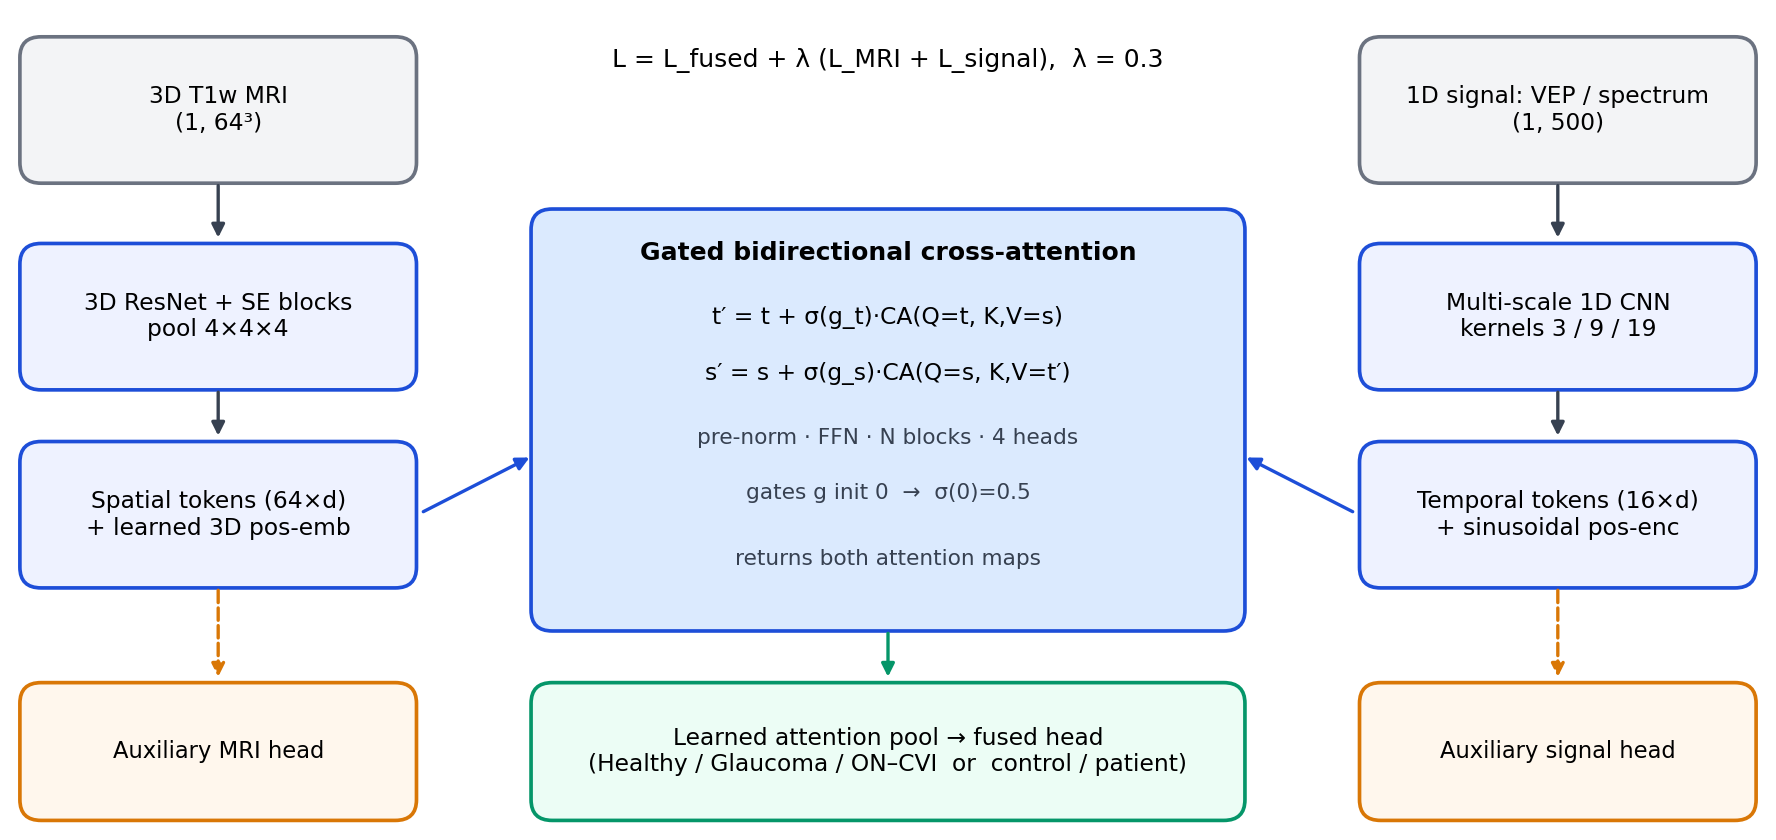
\includegraphics[width=0.66\textwidth]{figs/fig_arch_v2.png}
\caption{Data flow of CAFN. Preprocessed MRI and signal streams are encoded into spatial and temporal tokens, exchanged through gated bidirectional cross-attention, pooled by a learned attention pool and classified; two auxiliary heads read the unimodal tokens.}
\label{fig:pipeline}
\end{figure*}

\subsection{Preprocessing}\label{sec:mri}
\emph{MRI.} Volumes are reoriented to RAS, resampled to 1\,mm isotropic spacing and masked. Two foreground masks are implemented: an intensity-percentile mask (the original lightweight stand-in) and an Otsu threshold with hole filling and largest-component clean-up. For real whole-head T1w scans the volume is cropped to the foreground bounding box, resampled to $64^3$ (or $32^3$ for the cross-validation study), and normalised by a foreground z-score. A centre crop to $64^3$, which suffices for the small synthetic volumes, would see only a sliver of a 170\,mm head. Neither mask is a substitute for validated skull-stripping \cite{isensee2019,hoopes2022}.

\emph{VEP.} Records are validated, band-passed (4th-order Butterworth, 1--100\,Hz), notched at 50\,Hz ($Q=30$), both applied forward and backward so that the effective response is zero-phase,
\begin{equation}
H_{\mathrm{zp}}(\omega)=\lvert H(j\omega)\rvert^{2},\qquad \arg H_{\mathrm{zp}}(\omega)=0,
\end{equation}
resampled to 500 samples and z-scored. P100 latency is therefore not shifted.

\emph{Spectrum mode (real cohorts).} The public cohorts contain resting MEG or EEG, not VEPs. Each recording is reduced to the channel-averaged $\log_{10}$ Welch power spectral density between 1 and 45\,Hz, interpolated to 500 points and z-scored; the temporal encoder then operates on the spectrum and no time-domain filtering is applied.

\subsection{Encoders}
The spatial encoder is a stem (Conv3d, batch norm, ReLU) followed by three residual blocks (16$\to$32$\to$64$\to$128 channels, stride 2), each with a squeeze-and-excitation gate (reduction 4) \cite{hu2018}, and an adaptive average pool to $4\times4\times4$ giving $X_s\in\mathbb{R}^{64\times d}$ plus a learned 3D positional embedding. The temporal encoder is a stem followed by three strided stages, each followed by a \emph{multi-scale residual} block of parallel convolutions with kernels 3, 9 and 19, so that both a narrow peak and a broad waveform complex are visible; an adaptive pool gives 16 tokens $X_t\in\mathbb{R}^{16\times d}$ plus a sinusoidal positional encoding. All adaptive pooling is implemented as a per-axis matrix product with the exact PyTorch window weights; this is numerically equal to \texttt{AdaptiveAvgPool} but deterministic on CUDA and supported on Apple MPS.

\subsection{Gated bidirectional cross-attention}
In the original design only spatial tokens queried temporal tokens. CAFN now updates \emph{both} streams in each of $N$ pre-norm blocks, temporal first so that the spatial read consumes the enriched temporal tokens:
\begin{align}
t' &= t + \sigma(g_t)\,\mathrm{CA}\big(\mathrm{LN}(t),\,s\big),\quad t'\leftarrow t'+\mathrm{FFN}_t(\mathrm{LN}(t')),\\
s' &= s + \sigma(g_s)\,\mathrm{CA}\big(\mathrm{LN}(s),\,t'\big),\quad s'\leftarrow s'+\mathrm{FFN}_s(\mathrm{LN}(s')),
\end{align}
where $\mathrm{CA}(q,kv)$ is multi-head scaled dot-product attention with queries from $q$ and keys and values from $kv$,
\begin{equation}
\mathrm{CA}=\mathrm{softmax}\!\Big(\frac{QK^{\top}}{\sqrt{d_h}}\Big)V,\qquad d_h=d/H,
\end{equation}
and $g_s,g_t$ are learned scalar gates initialised at zero ($\sigma(0)=0.5$: both directions start half open). The fused spatial tokens are layer-normalised and pooled with a learned attention pool whose near-zero initial scorer reproduces mean pooling at the start of training.

\subsection{Objective and baselines}
Three linear heads read the pooled fused tokens, the mean spatial tokens and the mean temporal tokens. With cross-entropy losses $L_f,L_s,L_t$, $L=L_f+\lambda(L_s+L_t)$ with $\lambda=0.3$; class weights (inverse frequency) and label smoothing are optional. For like-for-like comparison we implement the fusion strategies used in the literature \cite{zhou2024camf}: \emph{concatenation} (mean-pooled streams concatenated and projected), \emph{element-wise sum}, and the two unimodal references (\emph{MRI only}, \emph{VEP/spectrum only}); all share the encoders, the auxiliary loss and the training recipe. The original one-way fusion with mean pooling and no positional encoding or SE is the \emph{v1-style} configuration.

\subsection{Explainability}
3D Grad-CAM (and Grad-CAM++) is computed on the last residual block from the fused logit, and the attention tensors of both directions are returned for plotting per head. A P100 latency estimator with an ISCEV-aligned search window converts the VEP stream into a clinician-checkable number. These are inspection aids, not clinical evidence.

\subsection{Controlled synthetic generator}\label{sec:synth}
A seeded generator produces class-conditioned MRI volumes (an ellipsoidal brain with ventricles; Glaucoma: a focal hypointensity, Optic Neuritis/CVI: a focal hyperintensity at a random location) and VEP records (N75--P100--N145 complex with class-specific latency and amplitude drawn per subject: $100\pm3$\,ms/$6.0\pm0.8$, $104\pm4$\,ms/$2.5\pm0.6$ and $138\pm6$\,ms/$4.0\pm1.0$ for the three classes, plus drift, mains and muscle noise). Two parameters, $\mu_{\mathrm{MRI}},\mu_{\mathrm{VEP}}\in[0,1]$, scale how far the lesion contrast and the VEP latency and amplitude offsets move from the healthy class (1: default generator; 0: no class signal). Because the two modalities are generated independently given the label, their evidence is complementary by construction; this is the setting in which fusion \emph{should} help, and the study asks how reliably each architecture exploits it.

\section{Experimental Setup}\label{sec:setup}
\subsection{Implementation and reproducibility}
CAFN is implemented in PyTorch \cite{paszke2019} with MONAI \cite{cardoso2022}, NiBabel, MNE-Python \cite{gramfort2013}, SciPy \cite{virtanen2020} and scikit-learn. All randomness derives from one constant seed (42; repeat $k$ uses $42{+}k$), deterministic algorithms are requested, and a single script (\texttt{run\_all.sh}) performs download, preprocessing, training, validation and testing and records the environment. Neural models were trained on an NVIDIA RTX 3050 Laptop GPU (4\,GB) with mixed precision; the model needs under 1\,GB at batch size 8. To finish in time, some synthetic runs were distributed over an Apple M3 Max (CPU or MPS) and the host CPU; every run is reproducible on its own device at a fixed seed, but results are not bit-identical across devices; all configurations of a given seed ran on the same device, so the paired comparisons between configurations are not affected.

\subsection{Study A: controlled synthetic benchmark}
Each (setting, seed) draws 144 training, 48 validation and 120 test samples (test drawn from a different seed range), $32^3$ MRI volumes and 500-point VEPs; checkpoints are selected on validation balanced accuracy and \emph{all} reported numbers are on the test set. The main setting ($\mu_{\mathrm{MRI}}=1.0$, $\mu_{\mathrm{VEP}}=0.3$) was fixed from a pilot that trained only the two unimodal models and chose the difficulty at which both were clearly above chance and below saturation; it was not tuned on CAFN. Twelve configurations (Table~\ref{tab:ablation}) are run on at least five seeds (more for the five key comparisons). A sweep varies $\mu_{\mathrm{VEP}}$ (MRI fixed) for four methods.

\subsection{Study B: real cohorts}
Two public OpenNeuro datasets with a patient group, a control group, a T1-weighted MRI and a resting recording are used (Table~\ref{tab:cohorts}): ds003568 (major depressive disorder vs healthy adolescents, MEG) \cite{liuzzi2022ds003568} and ds007181 (zoster-associated neuralgia vs healthy controls, whole-night polysomnographic EEG) \cite{ds007181}. Only subjects with both a T1w scan and a usable recording are kept (95 of 117 listed). The label is pan-disorder (0 control, 1 patient), which is a deliberate and important limitation.

\begin{table}[!t]
\caption{Real cohorts used (subjects with both modalities).}
\label{tab:cohorts}
\centering\scriptsize\setlength{\tabcolsep}{3pt}
\begin{tabular}{@{}lllrr@{}}
\toprule
Cohort & Patients vs controls & Signal & Ctrl & Pat\\
\midrule
ds003568 & MDD vs healthy & resting MEG (CTF) & 18 & 29\\
ds007181 & Zoster neuralgia vs healthy & PSG EEG & 27 & 21\\
\bottomrule
\end{tabular}
\end{table}

\emph{Protocols.} (i) \emph{Cohort split}: each cohort is split 70/15/15 (train/val/test); a pooled model is reported per cohort, and \emph{leave-one-cohort-out} (LODO) trains on one cohort and tests on every subject of the other. (ii) \emph{Repeated cross-validation}: every subject is predicted out-of-fold in 5-fold CV stratified on cohort and label, repeated five times for classical models and once for the neural models, so metrics use all 95 subjects instead of the 7-subject test splits. Classical baselines are logistic regression on the 500-point spectrum, on five band powers (delta 1--4, theta 4--8, alpha 8--13, beta 13--30, gamma 30--45\,Hz) and on PCA-reduced MRI ($8^3$ voxels $\to$ 20 components), a random forest on band powers, and MRI plus band powers. Neural variants (CAFN, concatenation, MRI only, spectrum only) use a regularised configuration ($d_{\mathrm{model}}=64$, dropout 0.3, weight decay $10^{-2}$) fixed in advance. (iii) \emph{Statistics}: ROC-AUC and balanced accuracy, a 1000-resample bootstrap 95\% interval over subjects, and a 200-permutation test that shuffles labels \emph{within} each cohort (preserving cohort base rates, so a cohort-identity shortcut cannot produce significance).

\subsection{Metrics}
Accuracy, macro-F1 and balanced accuracy for the three-class synthetic task; ROC-AUC and balanced accuracy for the binary real task. Differences between methods on the synthetic study are paired over seeds.
